\documentclass[10pt]{article}

\usepackage[margin=0.72in]{geometry}
\usepackage{amsmath,amssymb}
\usepackage{array}
\usepackage{booktabs}
\usepackage{caption}
\usepackage{enumitem}
\usepackage{eso-pic}
\usepackage{float}
\usepackage{graphicx}
\usepackage{hyperref}
\usepackage{longtable}
\usepackage{microtype}
\usepackage{multirow}
\usepackage{pdflscape}
\usepackage{placeins}
\usepackage{tabularx}
\usepackage{xcolor}

\hypersetup{
  colorlinks=true,
  linkcolor=blue!55!black,
  urlcolor=blue!55!black
}
\captionsetup{font=small,labelfont=bf}
\setlist[itemize]{leftmargin=1.35em,itemsep=0.25em,topsep=0.3em}
\setlist[enumerate]{leftmargin=1.5em,itemsep=0.3em,topsep=0.3em}
\setlength{\parindent}{0pt}
\setlength{\parskip}{0.48em}
\renewcommand{\arraystretch}{1.10}
\makeatletter
\setlength{\@fptop}{0pt}
\makeatother

\newcommand{\Rmodel}{R_{\mathrm{model}}}
\newcommand{\Gplus}{G^+_\kappa}
\newcommand{\Gpm}{G^\pm_\kappa}

\title{\textbf{S1 Ablation Study for Activation Sparsity in Pythia-14M}\\
\large Architecture, threshold gates, learned thresholds, pressure, and seed sensitivity}
\author{Thiago Mattar\\\texttt{thiagocmattar@gmail.com}}
\date{July 27, 2026}

\begin{document}
\maketitle

\begin{quote}
\textbf{Answer in brief.}
\begin{itemize}
  \item \textbf{Topology sets reach.} At the common AdamW setting,
  \(\Rmodel\) rises from effectively 0\% for stock A0 to 5.80\% for the
  Three-ReLU A3 path and 13.64\% for A6-POST. Adding V to matched Q/K parents
  contributes about 3.77 percentage points (pp) for less than 0.002 loss.
  \item \textbf{Thresholds expose a controllable tradeoff.} Increasing fixed
  \(\kappa\) raises \(\Rmodel\) in every complete A5/A6 ladder, with a small
  but nonzero loss cost. Signed \(G^\pm\) gates preserve lower loss than
  one-sided \(G^+\) gates, but give up 1.64--6.61 \(\Rmodel\) pp. Learned
  absolute thresholds add opportunity in all 15 matched fixed-threshold
  contrasts; RMS-relative learning instead shifts toward lower loss and lower
  opportunity.
  \item \textbf{Pressure and orthogonalization are distinct controls.}
  OL1/OR have lower loss than their exact naive partners in all 20 seed-0
  comparisons, but generally produce a smaller sparsity response. The 0.5
  orthogonal-step cap binds at every logged A6-POST update, so these are
  results for a budget-constrained procedure.
  \item \textbf{The evidence is screening evidence.} One coupled seed change
  preserves all ten logical-compute effect signs and nine of ten loss-effect
  signs. S1 supports a matched scale-up panel; it does not establish variance,
  model-scale generality, sparse-kernel speedup, or a global winner.
\end{itemize}
\end{quote}

\section{Scope and Scientific Questions}

\begin{table}[H]
\centering
\small
\caption{S1 experimental blocks. Every cell is a 2,048-step randomly
initialized Pythia-14M pretraining run; block-local departures from the common
contract are stated in the setup column.}
\label{tab:scope}
\begin{tabularx}{\textwidth}{p{0.11\textwidth} X X p{0.22\textwidth}}
\toprule
Block & Scientific question & Controlled setup & Primary comparison \\
\midrule
B0 & How do ordinary-ReLU topology and model learning rate change quality and
logical opportunity? & AdamW, no pressure; ten topologies; three LRs for five
anchors; 20 cells. & Direct topology parent and within-architecture LR. \\
B1 & How do fixed threshold, gate family, PRE/POST placement, and gated
topology change quality and logical opportunity? & AdamW at
\(3\times10^{-5}\); A1-H through A6 variants; 36 positive-threshold cells.
& Absolute endpoints by architecture, gate, and \(\kappa\), including
registered \(\kappa=0\) controls. \\
B2 & Does learned \(\kappa\) move beyond fixed \(\kappa=0.10\), and how do
score scale and threshold parameterization matter? & AdamW without pressure;
26 cells spanning architecture, gate, absolute/RMS-relative score, and three
parameterizations. & Absolute endpoints for fixed versus learned and absolute
versus RMS-relative thresholds. \\
B3 & How do pressure family, orthogonalization, weight, and Ricker geometry
change matched quality and opportunity? & A3 and A6-POST; all active gates;
orthogonal variants use fixed step budget 0.5. & Pressure--AdamW and
orthogonal--naive; 40 cells. \\
B4 & Which selected endpoints and effect directions survive one coupled seed
change? & Ten sentinels; initialization/data-order seeds \(0/0\) versus
\(1/1\). & Endpoint shifts and within-seed sign agreement. \\
\bottomrule
\end{tabularx}
\end{table}

S1 contains 132 completed scientific cells and 36 pooled diagnostics. Two
declared post-PV context-gate cells remained dependency-gated. The study is a
mostly one-seed feasibility screen on one frozen selection set: comparisons
are local and prespecified, no equivalence margin or multiplicity correction
was defined, and no global S1 rank is treated as confirmatory.

\section{Common Experimental Setup and Metrics}

\begin{table}[H]
\centering
\small
\caption{Common S1 experimental contract. A cache-pass equivalent is a token
ratio, not unique-token coverage or an epoch, because blocks are sampled with
replacement.}
\label{tab:contract}
\begin{tabularx}{\textwidth}{>{\bfseries}p{0.22\textwidth} X}
\toprule
Item & Frozen setting \\
\midrule
Model & Randomly initialized \texttt{EleutherAI/pythia-14m-deduped}; released
weights are not loaded. Six parallel-residual blocks, \(d=128\), MLP width
512, four heads, and sequence length 2,048. \\
Training data & MiniPile frozen train cache: 1,491,711,416 tokens. Random
contiguous blocks with replacement. \\
Budget and batching & 2,048 updates; 65,536 tokens/update; 134,217,728 tokens
per cell \(=0.089976\) cache-pass equivalents (8.998\%). Microbatch four
sequences, gradient accumulation eight, effective batch 32 sequences. \\
Optimizer & AdamW, \(\beta=(0.9,0.999)\), \(\epsilon=10^{-8}\), weight decay
0.01, no gradient clipping; 100-step linear warmup then constant LR. The common
LR is \(3\times10^{-5}\); only B0 has \(10^{-5}\) and \(10^{-4}\) flanks. \\
Validation & Frozen 250-document selection half of MiniPile validation:
311,739 cached tokens. Evaluation retains 152 complete sequences, 311,296
input positions, 38 batches, and discards 443 trailing tokens. Loss averages
311,144 shifted next-token targets. \\
Seeds and precision & Primary initialization/data-order seeds \(0/0\); B4
changes both to \(1/1\). FP32 parameters with bfloat16 autocast. \\
Execution and scale & Dense eager PyTorch on one NVIDIA GeForce RTX 5070 Ti
Laptop GPU (12,227 MiB). The 132 cells sum to 17.72B scheduled tokens and
50.76 scientific-run GPU-hours. No sparse kernel is used. \\
\bottomrule
\end{tabularx}
\end{table}

Pythia uses parallel attention and MLP residual branches. For residual input
\(H_\ell\), the relevant dataflow is
\[
[\widehat Q,\widehat K,\widehat V]=A_\ell W_{\mathrm{QKV}}+b_{\mathrm{QKV}},
\quad P=\operatorname{softmax}(QK^\top/\sqrt{d_h}+\mathcal M),
\quad C=PV,
\]
\[
H_{\ell+1}=H_\ell+(CW_o+b_o)+
  \bigl(\phi(M_\ell W_1+b_1)W_2+b_2\bigr),
\]
where active gates may transform the post-LayerNorm branch inputs
\(A_\ell,M_\ell\), MLP hidden \(h\), or post-projection Q/K/V. PRE gates act
on Q/K before RoPE; POST gates act after RoPE. The final model LayerNorm is
never gated.

The report uses two endpoint outcomes and one exact-zero counting convention:
\begin{itemize}
  \item \(L\): final step-2,048 selection next-token cross-entropy.
  \item An \emph{exact zero}: direct floating-point equality \(x=0\), with no
  tolerance. Counts are integer-pooled over the 152 validation sequences, all
  applicable coordinates, and all six layers.
  \item \(R_m\equiv\Rmodel\): the model-wide share of logical scalar products
  with at least one exact-zero activation operand in QKV, causal-valid QK,
  causal-valid PV, \(W_o\), \(W_1\), or \(W_2\). Future causal positions are
  excluded and the LM head is treated as dense.
\end{itemize}
Writing the exact-zero product count as \(Z\),
\[
\Rmodel=\frac{Z}
{857{,}085{,}050{,}880+2{,}004{,}407{,}549{,}952},
\]
where the first denominator term covers all six transformer blocks and the
second covers the LM head. \(R_m\) is a logical opportunity, not measured
FLOPs, latency, energy, or sparse-kernel speedup.

\begin{figure}[H]
\centering
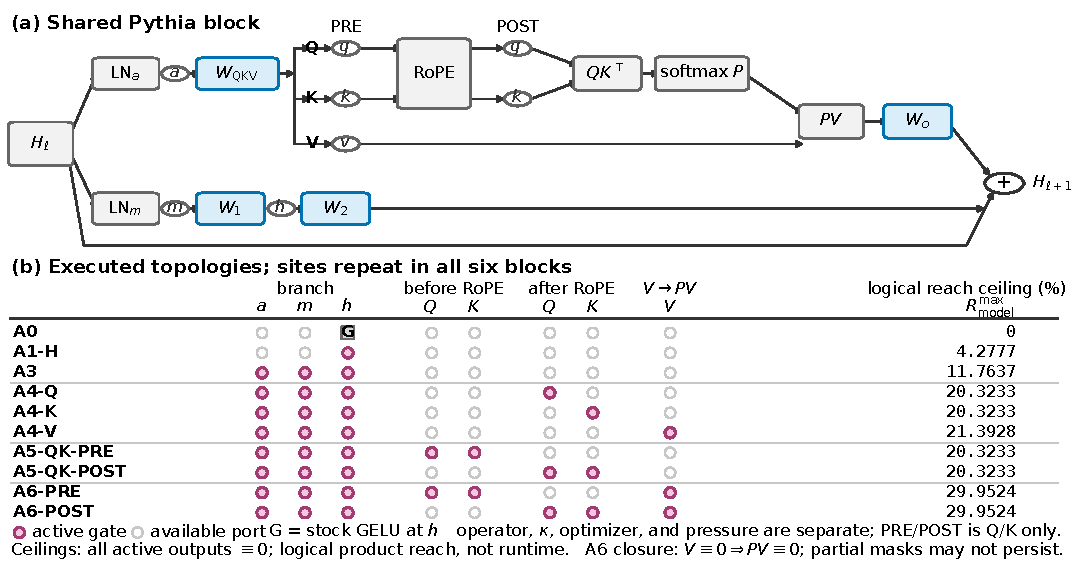
\includegraphics[width=\textwidth]{110-pythia-14m-s1-topology-atlas.pdf}
\caption{Pythia-14M topology atlas. Each row is one parallel-residual block;
filled gate markers show the exact-zero paths enabled by that architecture.
The right column gives the limiting model-wide reachable share under complete zeroing,
not the observed partial-mask values. PRE/POST refers to Q/K placement around
RoPE; V is always pre-PV.}
\label{fig:topology-atlas}
\end{figure}

\FloatBarrier
\section{Experimental Blocks}

\subsection{B0: Learning Rate and Architecture}

\textbf{Question and setup.} B0 asks how ordinary exact-zero paths and the
three tested model LRs change \(L\) and \(R_m\).
A0 retains stock GELU; every gated topology uses ordinary one-sided
\(G^+_0(x)=\max(x,0)\). All 20 cells use AdamW without activation pressure.

\begin{table}[H]
\centering
\footnotesize
\setlength{\tabcolsep}{4.2pt}
\caption{Complete B0 endpoints with learning rates in parallel column groups. Each group reports validation loss and $R_m$ (\%). All 20 cells use seed-0 AdamW for 2,048 steps without activation pressure. A0 uses stock GELU; gated architectures use ordinary $G^+_0$. A dash means that the architecture was not executed at that learning rate. Config IDs remain in the complete appendix.}
\label{tab:b0}
\begin{tabular}{l rr rr rr}
\toprule
\multirow{2}{*}{Architecture} & \multicolumn{2}{c}{$10^{-5}$} & \multicolumn{2}{c}{$3\times10^{-5}$} & \multicolumn{2}{c}{$10^{-4}$} \\
\cmidrule(lr){2-3}\cmidrule(lr){4-5}\cmidrule(lr){6-7}
& $L$ & $R_m$ (\%) & $L$ & $R_m$ (\%) & $L$ & $R_m$ (\%) \\
\midrule
A0 & 8.35104 & 0.00 & 7.04913 & 0.00 & 5.93887 & 0.00 \\
A1-H & 8.38652 & 1.97 & 6.98875 & 2.08 & 5.87474 & 2.40 \\
A3 & 8.40015 & 5.69 & 7.01310 & 5.80 & 5.91768 & 6.16 \\
A4-Q & \multicolumn{2}{c}{--} & 7.02126 & 7.71 & \multicolumn{2}{c}{--} \\
A4-K & \multicolumn{2}{c}{--} & 7.02441 & 8.28 & \multicolumn{2}{c}{--} \\
A4-V & \multicolumn{2}{c}{--} & 7.01615 & 9.50 & \multicolumn{2}{c}{--} \\
A5-QK-PRE & \multicolumn{2}{c}{--} & 7.01586 & 8.45 & \multicolumn{2}{c}{--} \\
A5-QK-POST & \multicolumn{2}{c}{--} & 7.03064 & 9.87 & \multicolumn{2}{c}{--} \\
A6-PRE & 8.38739 & 13.80 & 7.01645 & 12.22 & 5.93539 & 12.37 \\
A6-POST & 8.38743 & 14.83 & 7.03248 & 13.64 & 6.06320 & 13.64 \\
\bottomrule
\end{tabular}
\end{table}


\begin{figure}[H]
\centering
\includegraphics[width=\textwidth]{../../figures/112-pythia-14m-s1-learning-rate-effect.pdf}
\caption{B0 learning-rate response for the five registered anchor
architectures. All cells use AdamW without pressure. Panel (a) shows a
qualitatively shared monotone endpoint-loss response across the three tested
rates; panel (b) shows logical opportunity; panel (c) resolves the
\(10^{-4}\) architecture endpoints.}
\label{fig:b0}
\end{figure}

\textbf{Finding.} Relative to \(3\times10^{-5}\), \(10^{-5}\) raises loss by
1.3019--1.3978 for every anchor, while \(10^{-4}\) lowers it by
0.9693--1.1140. At the common LR, A4-V versus A3 adds 3.7030 \(R_m\) pp for
+0.00305 loss; adding V to the matched A5 PRE/POST parents adds
3.7735/3.7749 pp for +0.00059/+0.00184 loss. A6 PRE\(\rightarrow\)POST adds
1.4238 pp for +0.01603 loss.

\textbf{Limitation.} The LR result ranks step-2,048 endpoints only; it does not
identify a long-budget optimum. Topology comparisons expose logical reach,
not realized execution speed.

\FloatBarrier
\subsection{B1: Fixed Thresholds}

\textbf{Question and setup.} B1 studies two hard gate families,
\[
G^+_\kappa(x)=x\mathbf 1[x\ge\kappa],\qquad
G^\pm_\kappa(x)=x\mathbf 1[|x|\ge\kappa].
\]
The complete ladders are A5-QK-PRE, A5-QK-POST, A6-PRE-QKV, and
A6-POST-QKV with both gates and
\(\kappa\in\{0.03,0.10,0.30\}\). A4-Q/K/V isolate one projected tensor at
\(\kappa=0.10\). A1-H, A3, and A6-POST-ALL apply \(G^+_\kappa\) to every
active gate at \(\kappa\in\{0.03,0.10\}\); A6-POST-ALL therefore thresholds
\(a/m/h/Q/K/V\), whereas A6-POST-QKV thresholds only Q/K/V. Unlisted gates
remain ordinary ReLUs. \(G^+_0\) is ordinary ReLU; \(G^\pm_0\) is identity,
so the latter uses A3 as its registered zero-threshold control.

\begingroup
\footnotesize
\setlength{\tabcolsep}{3.4pt}
\renewcommand{\arraystretch}{1.03}
\begin{longtable}{l r r r r r r r}
\caption{Complete B1 endpoints with the two gate families in parallel column groups. Each group reports config, validation loss, and $R_m$ (\%). The 36 positive-threshold cells are shown with their registered $\kappa=0$ controls; repeated config IDs are shared controls. A6-POST-QKV thresholds Q/K/V, whereas A6-POST-ALL thresholds a/m/h/Q/K/V. $G^+_0$ is ordinary ReLU; $G^\pm_0$ is identity and uses A3 (config 125). A dash means that the gate family was not executed for that row. All cells use seed-0 AdamW at $3\times10^{-5}$ without pressure.}\label{tab:b1}\\
\toprule
\multirow{2}{*}{Architecture} & \multirow{2}{*}{$\kappa$} & \multicolumn{3}{c}{$G^+$} & \multicolumn{3}{c}{$G^\pm$} \\
\cmidrule(lr){3-5}\cmidrule(lr){6-8}
& & Cfg & $L$ & $R_m$ (\%) & Cfg & $L$ & $R_m$ (\%) \\
\midrule
\endfirsthead
\multicolumn{8}{c}{\tablename\ \thetable\ (continued)}\\
\toprule
\multirow{2}{*}{Architecture} & \multirow{2}{*}{$\kappa$} & \multicolumn{3}{c}{$G^+$} & \multicolumn{3}{c}{$G^\pm$} \\
\cmidrule(lr){3-5}\cmidrule(lr){6-8}
& & Cfg & $L$ & $R_m$ (\%) & Cfg & $L$ & $R_m$ (\%) \\
\midrule
\endhead
\bottomrule
\endlastfoot
\multirow{3}{*}{A1-H} & 0 & 124 & 6.98875 & 2.08 & \multicolumn{3}{c}{--} \\*
 & 0.03 & 204 & 6.98927 & 2.53 & \multicolumn{3}{c}{--} \\*
 & 0.10 & 205 & 6.99409 & 3.35 & \multicolumn{3}{c}{--} \\
\midrule
\multirow{3}{*}{A3} & 0 & 125 & 7.01310 & 5.80 & \multicolumn{3}{c}{--} \\*
 & 0.03 & 206 & 7.00780 & 6.61 & \multicolumn{3}{c}{--} \\*
 & 0.10 & 207 & 7.02685 & 7.93 & \multicolumn{3}{c}{--} \\
\midrule
\multirow{2}{*}{A4-Q} & 0 & 129 & 7.02126 & 7.71 & 125 & 7.01310 & 5.80 \\*
 & 0.10 & 197 & 7.02146 & 8.16 & 200 & 7.01355 & 6.49 \\
\midrule
\multirow{2}{*}{A4-K} & 0 & 130 & 7.02441 & 8.28 & 125 & 7.01310 & 5.80 \\*
 & 0.10 & 198 & 7.02413 & 9.06 & 201 & 7.01406 & 7.25 \\
\midrule
\multirow{2}{*}{A4-V} & 0 & 131 & 7.01615 & 9.50 & 125 & 7.01310 & 5.80 \\*
 & 0.10 & 199 & 7.01547 & 11.47 & 202 & 7.01501 & 9.92 \\
\midrule
\multirow{4}{*}{A5-QK-PRE} & 0 & 132 & 7.01586 & 8.45 & 125 & 7.01310 & 5.80 \\*
 & 0.03 & 149 & 7.01612 & 8.71 & 173 & 7.01319 & 6.56 \\*
 & 0.10 & 151 & 7.01905 & 9.88 & 175 & 7.01434 & 7.60 \\*
 & 0.30 & 153 & 7.03079 & 13.66 & 177 & 7.02590 & 12.00 \\
\midrule
\multirow{4}{*}{A5-QK-POST} & 0 & 133 & 7.03064 & 9.87 & 125 & 7.01310 & 5.80 \\*
 & 0.03 & 161 & 7.03029 & 10.15 & 185 & 7.01265 & 6.62 \\*
 & 0.10 & 163 & 7.03090 & 11.10 & 187 & 7.01402 & 7.83 \\*
 & 0.30 & 165 & 7.03559 & 13.77 & 189 & 7.02492 & 12.13 \\
\midrule
\multirow{4}{*}{A6-PRE-QKV} & 0 & 126 & 7.01645 & 12.22 & 125 & 7.01310 & 5.80 \\*
 & 0.03 & 155 & 7.01712 & 13.24 & 179 & 7.01432 & 7.90 \\*
 & 0.10 & 157 & 7.02195 & 15.70 & 181 & 7.01775 & 11.65 \\*
 & 0.30 & 159 & 7.03369 & 21.81 & 183 & 7.02352 & 19.14 \\
\midrule
\multirow{4}{*}{A6-POST-QKV} & 0 & 127 & 7.03248 & 13.64 & 125 & 7.01310 & 5.80 \\*
 & 0.03 & 167 & 7.03290 & 14.59 & 191 & 7.01313 & 7.98 \\*
 & 0.10 & 169 & 7.03408 & 16.91 & 193 & 7.01688 & 11.87 \\*
 & 0.30 & 171 & 7.03405 & 21.94 & 195 & 7.02043 & 19.51 \\
\midrule
\multirow{3}{*}{A6-POST-ALL} & 0 & 127 & 7.03248 & 13.64 & \multicolumn{3}{c}{--} \\*
 & 0.03 & 208 & 7.02389 & 15.44 & \multicolumn{3}{c}{--} \\*
 & 0.10 & 209 & 7.05266 & 18.61 & \multicolumn{3}{c}{--} \\
\end{longtable}
\endgroup


\begin{figure}[H]
\centering
\includegraphics[width=\textwidth]{../../figures/104-pythia-14m-s1-fixed-threshold-effect.pdf}
\caption{B1 threshold effect for the four complete A5/A6 ladders. Both panels
show absolute endpoints across \(\kappa\): validation loss and \(R_m\).
Colors identify architecture; solid circles and dashed open squares identify
\(G^+\) and \(G^\pm\). At \(\kappa=0\), \(G^+\) uses the same-architecture
ordinary-ReLU control and \(G^\pm\) uses the shared A3 identity control.}
\label{fig:b1-threshold}
\end{figure}

\begin{figure}[H]
\centering
\includegraphics[width=\textwidth]{../../figures/105-pythia-14m-s1-gate-type-effect.pdf}
\caption{B1 gate-type effect at matched positive thresholds. Each segment
connects the absolute \(G^+\) and \(G^\pm\) endpoints for one architecture
and \(\kappa\); panels show validation loss and \(R_m\), not paired
differences. Color identifies architecture and marker shape identifies
\(\kappa\).}
\label{fig:b1-gate}
\end{figure}

\begin{figure}[H]
\centering
\includegraphics[width=\textwidth]{../../figures/116-pythia-14m-s1-fixed-threshold-quality-opportunity-frontiers.pdf}
\caption{B1 architecture-conditioned quality--opportunity frontiers. Each
path follows the tested \(\kappa\) ladder from its registered zero-threshold
control; lower loss and larger \(R_m\) are favorable. Color identifies
architecture and line/marker style identifies gate family. These are observed
threshold paths, not a cross-architecture ranking.}
\label{fig:b1-frontier}
\end{figure}

\textbf{Finding.} In the four complete ladders, raising \(\kappa\) from 0.03
to 0.30 increases \(R_m\) in all eight architecture/gate combinations by
3.62--11.53 pp, with +0.00115--0.01657 loss. At each positive threshold,
\(G^\pm\) has lower loss than \(G^+\) in all 12 matched architecture--\(\kappa\)
pairs, but also 1.64--6.61 pp lower \(R_m\). Table~\ref{tab:b1} retains the
A1/A3/A4 and A6-POST-ALL endpoints without collapsing them into paired ranges.

\textbf{Limitation.} Absolute \(\kappa\) acts on heterogeneous activation
scales, especially in the all-active rows; topology and scale are not
separated. The mostly one-seed screen has no prespecified equivalence margin.

\FloatBarrier
\subsection{B2: Learned Thresholds}

\textbf{Question and setup.} B2 asks whether a learned positive threshold
improves on fixed \(\kappa=0.10\), and whether the threshold should use raw or
RMS-normalized activation magnitudes. The learned threshold is
\[
\kappa=\operatorname{softplus}(\rho),\qquad
s(x)=
\begin{cases}
x, & G^+,\\
|x|, & G^\pm.
\end{cases}
\]
Softplus keeps \(\kappa>0\). For a gate tensor with \(N\) elements, its
root-mean-square magnitude and comparison score are
\[
r(x)=\max\!\left(\sqrt{\frac{1}{N}\sum_i x_i^2},10^{-8}\right),\qquad
u(x)=
\begin{cases}
s(x), & \text{absolute},\\
s(x)/r(x), & \text{RMS-relative}.
\end{cases}
\]
Thus absolute thresholds use activation units, whereas RMS-relative thresholds
scale with the current full gate tensor. The forward pass remains a hard gate:
\[
y=x\,\mathbf 1[u(x)\ge\kappa].
\]
Masked values are therefore exact zeros. During training only, the derivative
of the threshold comparison is replaced by the sigmoid surrogate
\(\operatorname{sigmoid}((u(x)-\kappa)/\tau)\). The score and RMS are treated
as constants in that surrogate, so it updates \(\rho\) only; the input keeps
the hard-mask zero-or-one derivative.

All cells initialize \(\kappa=0.10\), use \(\tau=0.03\), and train thresholds
at \(3\times10^{-4}\) without weight decay; the model uses seed-0 AdamW at
\(3\times10^{-5}\) for 2,048 steps without activation pressure. ``Model-wide''
means one \(\kappa\) for every learned gate, ``per site'' means one for each of
Q/K/V shared across layers, and ``per layer/site'' means a separate \(\kappa\)
for every layer and gate site. A6-POST-QKV learns only Q/K/V while retaining
ordinary ReLUs at a/m/h; A6-POST-ALL learns a/m/h/Q/K/V.

\begingroup
\footnotesize
\setlength{\tabcolsep}{2.7pt}
\renewcommand{\arraystretch}{1.03}
\begin{longtable}{l l l r r r r r r}
\caption{Complete B2 endpoints with the two gate families in parallel column groups. Each group reports config, validation loss, and $R_m$ (\%). Rows specify architecture, score scale, and threshold parameterization. A6-POST-QKV learns thresholds only at Q/K/V; A6-POST-ALL learns them at a/m/h/Q/K/V. A dash means that the gate family was not executed for that row. All 26 cells use seed-0 AdamW at $3\times10^{-5}$ for 2,048 steps without activation pressure.}\label{tab:b2}\\
\toprule
\multirow{2}{*}{Architecture} & \multirow{2}{*}{Score scale} & \multirow{2}{*}{$\kappa$ parameters} & \multicolumn{3}{c}{$G^+$} & \multicolumn{3}{c}{$G^\pm$} \\
\cmidrule(lr){4-6}\cmidrule(lr){7-9}
& & & Cfg & $L$ & $R_m$ (\%) & Cfg & $L$ & $R_m$ (\%) \\
\midrule
\endfirsthead
\multicolumn{9}{c}{\tablename\ \thetable\ (continued)}\\
\toprule
\multirow{2}{*}{Architecture} & \multirow{2}{*}{Score scale} & \multirow{2}{*}{$\kappa$ parameters} & \multicolumn{3}{c}{$G^+$} & \multicolumn{3}{c}{$G^\pm$} \\
\cmidrule(lr){4-6}\cmidrule(lr){7-9}
& & & Cfg & $L$ & $R_m$ (\%) & Cfg & $L$ & $R_m$ (\%) \\
\midrule
\endhead
\bottomrule
\endlastfoot
\multirow{2}{*}{A1-H} & Absolute & Per layer/site & 237 & 7.00088 & 3.66 & \multicolumn{3}{c}{--} \\*
 & RMS-relative & Per layer/site & 238 & 6.99136 & 2.65 & \multicolumn{3}{c}{--} \\
\midrule
\multirow{2}{*}{A3} & Absolute & Per layer/site & 239 & 7.04232 & 8.14 & \multicolumn{3}{c}{--} \\*
 & RMS-relative & Per layer/site & 240 & 7.01449 & 6.90 & \multicolumn{3}{c}{--} \\
\midrule
\multirow{2}{*}{A5-QK-PRE} & Absolute & Per layer/site & 221 & 7.01955 & 10.54 & 222 & 7.01458 & 8.29 \\*
 & RMS-relative & Per layer/site & 229 & 7.01594 & 9.56 & 230 & 7.01283 & 8.17 \\
\midrule
\multirow{2}{*}{A5-QK-POST} & Absolute & Per layer/site & 225 & 7.03098 & 11.63 & 226 & 7.01430 & 8.61 \\*
 & RMS-relative & Per layer/site & 233 & 7.03041 & 10.69 & 234 & 7.01226 & 8.49 \\
\midrule
\multirow{2}{*}{A6-PRE-QKV} & Absolute & Per layer/site & 223 & 7.02197 & 16.54 & 224 & 7.01763 & 12.71 \\*
 & RMS-relative & Per layer/site & 231 & 7.01330 & 13.95 & 232 & 7.01309 & 9.06 \\
\midrule
\multirow{4}{*}{A6-POST-QKV} & Absolute & Model-wide & 243 & 7.03386 & 17.76 & 245 & 7.01623 & 13.38 \\*
 & Absolute & Per site & 244 & 7.03378 & 18.14 & 246 & 7.01657 & 13.78 \\*
 & Absolute & Per layer/site & 227 & 7.03411 & 17.67 & 228 & 7.01617 & 13.09 \\*
 & RMS-relative & Per layer/site & 235 & 7.02936 & 14.96 & 236 & 7.01146 & 9.41 \\
\midrule
\multirow{2}{*}{A6-POST-ALL} & Absolute & Per layer/site & 241 & 7.06515 & 19.49 & \multicolumn{3}{c}{--} \\*
 & RMS-relative & Per layer/site & 242 & 7.03240 & 16.26 & \multicolumn{3}{c}{--} \\
\end{longtable}
\endgroup


\begin{figure}[H]
\centering
\includegraphics[width=\textwidth]{../../figures/106-pythia-14m-s1-learned-threshold-ablation.pdf}
\caption{B2 threshold effect for the 11 architecture/gate settings with one
threshold per layer/site. Each trajectory connects fixed \(\kappa=0.10\),
learned absolute, and learned RMS-relative endpoints. Both panels show
absolute validation loss and \(R_m\).}
\label{fig:b2-learned}
\end{figure}

\begin{table}[H]
\centering
\footnotesize
\setlength{\tabcolsep}{4.0pt}
\caption{Distribution of the final learned thresholds. All cells start from $\kappa=0.10$; values are read from the exact final checkpoint summaries. The mean pools threshold parameters: a run contributes one model-wide value, three site-shared values, or one value for every learned layer/site. Absolute and RMS-relative values live on different score scales and should not be compared as activation units.}
\label{tab:b2-kappa}
\begin{tabularx}{\textwidth}{X r r r r r}
\toprule
Threshold stratum & Runs & Parameters & Min. & Mean & Max. \\
\midrule
Q/K(/V), absolute, per layer/site & 8 & 120 & 0.1001 & 0.1444 & 0.2020 \\
Q/K(/V), RMS-relative, per layer/site & 8 & 120 & 0.1074 & 0.1581 & 0.2178 \\
a/m/h, absolute, per layer/site & 3 & 60 & 0.0839 & 0.1318 & 0.1997 \\
a/m/h, RMS-relative, per layer/site & 3 & 60 & 0.0942 & 0.1543 & 0.2143 \\
A6-POST Q/K/V, absolute, model-wide & 2 & 2 & 0.1328 & 0.1329 & 0.1329 \\
A6-POST Q/K/V, absolute, per site & 2 & 6 & 0.1306 & 0.1552 & 0.1924 \\
\bottomrule
\end{tabularx}
\end{table}


\textbf{Finding.} In the 11 per-layer/site comparisons, learning an absolute
threshold raises \(R_m\) by 0.21--1.21 pp relative to fixed \(\kappa=0.10\),
while loss moves by -0.00071 to +0.01546. RMS-relative scoring lowers loss by
0.00057--0.03275 and \(R_m\) by 0.13--3.67 pp relative to learned absolute
scoring in all 11 comparisons. For A6-POST-QKV with absolute scoring, the three
threshold parameterizations span less than 0.0004 loss and 0.70 \(R_m\) pp;
Table~\ref{tab:b2} retains all 26 endpoints. The exact final threshold
summaries in Table~\ref{tab:b2-kappa} show nontrivial movement from the common
0.10 initialization: stratum means span 0.1318--0.1581 and individual values
span 0.0839--0.2178.

\textbf{Limitation.} Thresholds optimize task loss, not sparsity. No fixed
RMS-relative control exists, only A6-POST-QKV tests all three threshold
parameterizations, and the screen has one seed.

\FloatBarrier
\subsection{B3: Pressure and Orthogonalization}

\textbf{Question and setup.} For active tensors \(s\in\mathcal S\), pressure
first averages scalars within a tensor and then weights tensors equally:
\[
\mathcal L_{\mathrm{L1}}=\frac1{|\mathcal S|}\sum_s\frac1{N_s}\sum_i|x_{s,i}|,
\quad
\mathcal L_{\mathrm R}=1-\frac1{|\mathcal S|}\sum_s\frac1{N_s}\sum_i
\left(1-\frac{x_{s,i}^2}{c^2}\right)e^{-x_{s,i}^2/(2\sigma^2)}.
\]
L1N/RN add weighted pressure to the training loss. OL1/OR instead apply the
pressure correction after the AdamW task step, removing the component that
conflicts with that task step. Their pressure/task update ratio is capped at
0.5 as a fixed stability control. In the Ricker pressure, \(c\) is the
zero-crossing scale and \(\sigma\) controls the envelope width. The promotion
guardrail remains
\(L_{\mathrm{method}}-L_{\text{same-architecture AdamW}}\le0.05\); it is an
evaluation rule, not a training objective.

\paragraph{Pressure weight and orthogonalization.}
B3 crosses A3 and A6-POST with L1 weights \(\{0.15,1,5\}\) and Ricker weights
\(\{0.1,0.3,1\}\), fixing \(c=\sigma=0.10\) for the Ricker weight sweep.

\begingroup
\scriptsize
\setlength{\tabcolsep}{2.1pt}
\renewcommand{\arraystretch}{1.03}
\begin{longtable}{l l r r r r r r r r r r}
\caption{Complete B3 pressure-weight endpoints. Each method group reports config, validation loss, and $R_m$ (\%). L1 rows compare L1N with OL1; Ricker rows compare RN with OR at $c=\sigma=0.10$. AdamW is the matched same-architecture control. All cells use seed 0 and 2,048 steps.}\label{tab:b3-weight}\\
\toprule
\multirow{2}{*}{Architecture} & \multirow{2}{*}{Pressure} & \multirow{2}{*}{$w$} & \multicolumn{3}{c}{AdamW} & \multicolumn{3}{c}{Naive} & \multicolumn{3}{c}{Orthogonal} \\
\cmidrule(lr){4-6}\cmidrule(lr){7-9}\cmidrule(lr){10-12}
& & & Cfg & $L$ & $R_m$ (\%) & Cfg & $L$ & $R_m$ (\%) & Cfg & $L$ & $R_m$ (\%) \\
\midrule
\endfirsthead
\multicolumn{12}{c}{\tablename\ \thetable\ (continued)}\\
\toprule
\multirow{2}{*}{Architecture} & \multirow{2}{*}{Pressure} & \multirow{2}{*}{$w$} & \multicolumn{3}{c}{AdamW} & \multicolumn{3}{c}{Naive} & \multicolumn{3}{c}{Orthogonal} \\
\cmidrule(lr){4-6}\cmidrule(lr){7-9}\cmidrule(lr){10-12}
& & & Cfg & $L$ & $R_m$ (\%) & Cfg & $L$ & $R_m$ (\%) & Cfg & $L$ & $R_m$ (\%) \\
\midrule
\endhead
\bottomrule
\endlastfoot
\multirow{6}{*}{A3} & \multirow{3}{*}{L1} & 0.15 & 125 & 7.01310 & 5.80 & 257 & 7.02421 & 5.07 & 258 & 7.01421 & 5.13 \\*
 &  & 1 & 125 & 7.01310 & 5.80 & 248 & 7.05338 & 4.59 & 249 & 7.02002 & 4.69 \\*
 &  & 5 & 125 & 7.01310 & 5.80 & 261 & 7.17578 & 5.18 & 262 & 7.02909 & 4.71 \\*
 & \multirow{3}{*}{Ricker} & 0.1 & 125 & 7.01310 & 5.80 & 266 & 7.03683 & 7.23 & 267 & 7.03121 & 7.28 \\*
 &  & 0.3 & 125 & 7.01310 & 5.80 & 252 & 7.10085 & 8.16 & 253 & 7.04616 & 7.87 \\*
 &  & 1 & 125 & 7.01310 & 5.80 & 270 & 7.20123 & 8.77 & 271 & 7.05883 & 8.25 \\
\midrule
\multirow{6}{*}{A6-POST} & \multirow{3}{*}{L1} & 0.15 & 127 & 7.03248 & 13.64 & 259 & 7.04048 & 18.77 & 260 & 7.03898 & 17.70 \\*
 &  & 1 & 127 & 7.03248 & 13.64 & 250 & 7.05312 & 19.60 & 251 & 7.03895 & 17.69 \\*
 &  & 5 & 127 & 7.03248 & 13.64 & 263 & 7.09562 & 21.32 & 264 & 7.03870 & 17.70 \\*
 & \multirow{3}{*}{Ricker} & 0.1 & 127 & 7.03248 & 13.64 & 268 & 7.05868 & 21.88 & 269 & 7.03926 & 17.55 \\*
 &  & 0.3 & 127 & 7.03248 & 13.64 & 254 & 7.09617 & 23.67 & 255 & 7.03930 & 17.56 \\*
 &  & 1 & 127 & 7.03248 & 13.64 & 272 & 7.16248 & 24.90 & 273 & 7.03909 & 17.56 \\
\end{longtable}
\endgroup


\begin{figure}[H]
\centering
\includegraphics[width=\textwidth]{../../figures/107-pythia-14m-s1-pressure-weight-ablation.pdf}
\caption{B3 pressure-weight response. Each trajectory starts at the matched
AdamW control and continues through the three pressure weights. Panels show
absolute validation loss and \(R_m\). Color and marker identify naive versus
orthogonal pressure; line style identifies A3 versus A6-POST. L1 and Ricker
weights are separate axes because their objective scales differ.}
\label{fig:b3-weight}
\end{figure}

\begin{figure}[H]
\centering
\includegraphics[width=\textwidth]{../../figures/118-pythia-14m-s1-pressure-quality-opportunity-frontiers.pdf}
\caption{B3 pressure-weight quality--opportunity frontiers. Each path begins
at its matched AdamW control and then follows one L1N, OL1, RN, or OR weight
ladder; lower loss and larger \(R_m\) are favorable. L1 and Ricker weights
index different objectives and are not numerically interchangeable.}
\label{fig:b3-frontier}
\end{figure}

\textbf{Finding.} The orthogonal method has lower loss than its matched naive
method in all 12 weight comparisons, but it does not preserve the full naive
\(R_m\) gain. On A6-POST, OL1 changes by less than 0.0003 loss and 0.002
\(R_m\) pp across its weight ladder; OR changes by less than 0.0003 loss and
0.011 pp. The corresponding naive ladders remain weight-sensitive. This flat
A6 orthogonal response coincides with the update-ratio cap binding on every
logged orthogonal update.

\paragraph{Ricker geometry.}
The geometry screen fixes \(w=0.30\). One sweep couples
\(c=\sigma\in\{0.05,0.10,0.50\}\); the other fixes \(c=0.10\) and varies
\(\sigma\in\{0.05,0.10,0.20\}\).

\begingroup
\scriptsize
\setlength{\tabcolsep}{2.1pt}
\renewcommand{\arraystretch}{1.03}
\begin{longtable}{l l r r r r r r r r r r}
\caption{Complete B3 Ricker-geometry endpoints at $w=0.30$. Each method group reports config, validation loss, and $R_m$ (\%). The basin sweep couples $c=\sigma$; the shape sweep fixes $c=0.10$ and varies $\sigma$. AdamW is the matched same-architecture control.}\label{tab:b3-geometry}\\
\toprule
\multirow{2}{*}{Architecture} & \multirow{2}{*}{Sweep} & \multirow{2}{*}{Value} & \multicolumn{3}{c}{AdamW} & \multicolumn{3}{c}{RN} & \multicolumn{3}{c}{OR} \\
\cmidrule(lr){4-6}\cmidrule(lr){7-9}\cmidrule(lr){10-12}
& & & Cfg & $L$ & $R_m$ (\%) & Cfg & $L$ & $R_m$ (\%) & Cfg & $L$ & $R_m$ (\%) \\
\midrule
\endfirsthead
\multicolumn{12}{c}{\tablename\ \thetable\ (continued)}\\
\toprule
\multirow{2}{*}{Architecture} & \multirow{2}{*}{Sweep} & \multirow{2}{*}{Value} & \multicolumn{3}{c}{AdamW} & \multicolumn{3}{c}{RN} & \multicolumn{3}{c}{OR} \\
\cmidrule(lr){4-6}\cmidrule(lr){7-9}\cmidrule(lr){10-12}
& & & Cfg & $L$ & $R_m$ (\%) & Cfg & $L$ & $R_m$ (\%) & Cfg & $L$ & $R_m$ (\%) \\
\midrule
\endhead
\bottomrule
\endlastfoot
\multirow{6}{*}{A3} & \multirow{3}{*}{$c=\sigma$} & 0.05 & 125 & 7.01310 & 5.80 & 275 & 7.12042 & 8.36 & 276 & 7.03339 & 7.84 \\*
 &  & 0.1 & 125 & 7.01310 & 5.80 & 252 & 7.10085 & 8.16 & 253 & 7.04616 & 7.87 \\*
 &  & 0.5 & 125 & 7.01310 & 5.80 & 279 & 7.07964 & 7.32 & 280 & 7.05550 & 7.33 \\*
 & \multirow{3}{*}{$\sigma$ at $c=0.10$} & 0.05 & 125 & 7.01310 & 5.80 & 284 & 7.10143 & 8.68 & 285 & 7.05176 & 8.24 \\*
 &  & 0.1 & 125 & 7.01310 & 5.80 & 252 & 7.10085 & 8.16 & 253 & 7.04616 & 7.87 \\*
 &  & 0.2 & 125 & 7.01310 & 5.80 & 288 & 7.12562 & 8.09 & 289 & 7.04407 & 7.60 \\
\midrule
\multirow{6}{*}{A6-POST} & \multirow{3}{*}{$c=\sigma$} & 0.05 & 127 & 7.03248 & 13.64 & 277 & 7.10916 & 23.23 & 278 & 7.03514 & 17.02 \\*
 &  & 0.1 & 127 & 7.03248 & 13.64 & 254 & 7.09617 & 23.67 & 255 & 7.03930 & 17.56 \\*
 &  & 0.5 & 127 & 7.03248 & 13.64 & 281 & 7.07163 & 21.01 & 282 & 7.04037 & 18.10 \\*
 & \multirow{3}{*}{$\sigma$ at $c=0.10$} & 0.05 & 127 & 7.03248 & 13.64 & 286 & 7.09446 & 24.23 & 287 & 7.03708 & 17.39 \\*
 &  & 0.1 & 127 & 7.03248 & 13.64 & 254 & 7.09617 & 23.67 & 255 & 7.03930 & 17.56 \\*
 &  & 0.2 & 127 & 7.03248 & 13.64 & 290 & 7.11203 & 24.03 & 291 & 7.04009 & 17.85 \\
\end{longtable}
\endgroup


\begin{figure}[H]
\centering
\includegraphics[width=\textwidth]{../../figures/108-pythia-14m-s1-ricker-shape-ablation.pdf}
\caption{B3 Ricker-geometry response at \(w=0.30\). Each trajectory starts at
the matched AdamW control; the remaining points vary only the displayed
geometry parameter. Panels show absolute validation loss and \(R_m\). Color
and marker identify RN versus OR; line style identifies architecture.}
\label{fig:b3-geometry}
\end{figure}

\textbf{Finding.} Geometry interacts with both update rule and architecture.
Increasing the coupled basin from 0.05 to 0.50 lowers RN loss by 0.0408 on A3
and 0.0375 on A6-POST, while reducing \(R_m\) by 1.04 and 2.22 pp. For OR, the
same change raises A6-POST \(R_m\) by 1.08 pp but lowers A3 \(R_m\) by 0.51 pp.
The shape sweep is also non-monotone for RN. No single Ricker geometry
dominates across method and architecture.

\textbf{Limitation.} The screen has one seed and 2,048 steps. Tensors are
weighted equally rather than by width or matmul cost, so pressure does not
directly optimize \(R_m\). The cap also binds on 52.38\% of logged A3 central
updates and every logged A6-POST orthogonal update; these cells therefore
characterize the budgeted procedure, not unconstrained orthogonal geometry.

\FloatBarrier
\subsection{B4: Seed Sensitivity}

\textbf{Question and setup.} B4 repeats ten sentinels---A0, A1-H, A3,
A6-PRE, A6-POST, fixed \(G^+\), fixed \(G^\pm\), learned \(G^\pm\), L1N,
and OR---while jointly changing model-initialization and data-order seeds from
\(0/0\) to \(1/1\). Every other scientific field is fixed.

\begin{figure}[H]
\centering
\includegraphics[width=\textwidth]{../../figures/109-pythia-14m-s1-seed-sensitivity.pdf}
\caption{B4 seed sensitivity. Top: absolute seed-0/seed-1 endpoints. Bottom:
within-seed matched effects. Dashed lines are identity. The only loss-sign
reversal is labelled. The contrasts share controls and were selected after
the seed-0 screen.}
\label{fig:b4}
\end{figure}

\textbf{Finding.} All ten \(R_m\) effect signs and nine of ten loss-effect
signs agree. Seed-1 endpoint losses shift by +0.00631--0.02028; absolute
\(R_m\) shifts are at most 0.2094 pp. The sole reversal is fixed
\(G^\pm_{0.10}\) minus A3.

\textbf{Limitation.} This is a two-point coupled sensitivity check, not a
variance estimate or independent confirmation. Initialization and data-order
effects cannot be separated, and B4 has no seed-1 RN or OL1 cell.

\FloatBarrier
\section{Synthesis, Descriptive Frontier, and Next Step}

For descriptive context, the common-condition landscape retains every valid
seed-0 cell at model LR \(3\times10^{-5}\), the shared 2,048-step budget, and
the frozen selection set. This excludes ten B0 LR flanks and ten B4 seed-1
sentinels, leaving \(n=112\). Point \(j\) is nondominated when no eligible
point \(i\) satisfies
\[
L_i\le L_j,\qquad R_{m,i}\ge R_{m,j},
\]
with at least one strict inequality. This is an exact descriptive envelope,
not the promoted experimental panel.

\begin{figure}[H]
\centering
\includegraphics[width=\textwidth]{../../figures/113-pythia-14m-s1-quality-compute-endpoint-landscape.pdf}
\caption{S1 quality--compute landscape. Panel (a) shows all 132 scientific
endpoints and therefore mixes learning rates and seeds. Panel (b) restricts
to the primary-seed common-LR cohort and labels the exact nondominated
envelope F1--F13. Architecture ceilings differ, so cross-topology \(R_m\)
must be read against gate scope and matched controls.}
\label{fig:landscape}
\end{figure}

\begin{table}[H]
\centering
\footnotesize
\setlength{\tabcolsep}{4.5pt}
\caption{Exact members of the descriptive nondominated envelope in Figure~\ref{fig:landscape}. The eligible cohort fixes model/data-order seeds at 0/0, model LR at $3\times10^{-5}$, the 2,048-step budget, and the frozen selection partition ($n=112$). F12--F13 exceed the predeclared $+0.05$ pressure-loss guardrail and are descriptive, not promotion choices.}
\label{tab:frontier}
\begin{tabularx}{\textwidth}{c r c X r r}
\toprule
ID & Cfg & Block & Design & $L$ & $R_m$ (\%) \\
\midrule
F1 & 124 & B0 & A1-H AdamW & 6.98875 & 2.08 \\
F2 & 204 & B1 & A1-H $G^+$, $\kappa=0.03$ & 6.98927 & 2.53 \\
F3 & 238 & B2 & A1-H ATG $G^+$, RMS, PLS & 6.99136 & 2.65 \\
F4 & 205 & B1 & A1-H $G^+$, $\kappa=0.10$ & 6.99409 & 3.35 \\
F5 & 237 & B2 & A1-H ATG $G^+$, ABS, PLS & 7.00088 & 3.66 \\
F6 & 206 & B1 & A3 $G^+$, $\kappa=0.03$ & 7.00780 & 6.61 \\
F7 & 236 & B2 & A6-POST ATG $G^\pm$, RMS, PLS & 7.01146 & 9.41 \\
F8 & 231 & B2 & A6-PRE ATG $G^+$, RMS, PLS & 7.01330 & 13.95 \\
F9 & 195 & B1 & A6-POST $G^\pm$, $\kappa=0.30$ & 7.02043 & 19.51 \\
F10 & 159 & B1 & A6-PRE $G^+$, $\kappa=0.30$ & 7.03369 & 21.81 \\
F11 & 171 & B1 & A6-POST $G^+$, $\kappa=0.30$ & 7.03405 & 21.94 \\
F12 & 286 & B3 & A6-POST RN, $(w,c,\sigma)=(0.3,0.1,0.05)$ & 7.09446 & 24.23 \\
F13 & 272 & B3 & A6-POST RN, $(w,c,\sigma)=(1,0.1,0.1)$ & 7.16248 & 24.90 \\
\bottomrule
\end{tabularx}
\end{table}


Three conclusions survive the blockwise controls:
\begin{itemize}
  \item \textbf{Architecture precedes optimization.} Gate placement defines
  which operands can be zero. V and POST Q/K enlarge observed opportunity,
  while projections,
  attention aggregation, and residual addition regenerate dense values.
  \item \textbf{Thresholds and pressure are different controls.} Fixed and
  learned gates set forward support directly. Pressure reshapes activation
  distributions, and orthogonalization changes how much task damage the
  pressure update accepts. Their weights and endpoints are not interchangeable.
  \item \textbf{The global envelope is descriptive.} F12--F13 obtain the
  largest \(R_m\) through RN but violate the predeclared +0.05 pressure-loss
  guardrail. Matched controls required for causal comparison need not lie on
  the envelope.
\end{itemize}

The next rung should freeze a matched panel before observing new data: A0, A3,
and ordinary A6-PRE/A6-POST controls; fixed POST-QKV \(G^+_{0.10}\) and
\(G^\pm_{0.10}\), plus high-opportunity \(G^+_{0.30}\); learned absolute
\(G^\pm\) with one threshold per layer/site; and matched L1N/OL1 and RN/OR
anchors. First extend the Pythia-14M
token budget under the frozen ladder: S2 uses seeds 0/1 on the selection
partition; S3 uses fresh seeds 2--4 on the document-disjoint
campaign-confirmation partition. That partition is not untouched, so
claim-grade confirmation still requires a new independent evaluation source.
Then scale the frozen panel across the Pythia family, recomputing topology
ceilings at each size. Freeze topology and gate family, but do not assume that
absolute \(\kappa\) or Ricker \((c,\sigma)\) transfers across activation
scales; predeclare a normalized transfer or report frozen and retuned curves
separately. Sparse-kernel latency, energy, masking, indexing, RoPE, softmax,
and residual overhead should be measured only after the logical frontier is
stable.

\section{Reproducibility and Provenance}

The data-derived figures, tables, and provenance sidecar are regenerated from
the applied config/run registries by:
\begin{verbatim}
make plot-report07
\end{verbatim}
On the recorded Windows host, the directly executable equivalent is
\texttt{mingw32-make plot-report07}.
The canonical PDF is then compiled by running
\texttt{pdflatex 07-2026-07-27-s1-ablation-study.tex} twice from the report
directory. The plotting target generates the topology atlas, Figures 103--110,
112--114, 116, and 118, the frontier table, the 132-row appendix, PNG previews,
and the provenance sidecar. The registry-driven generators validate the expected
20/36/26/40/10 block counts and the 311,296-position propagation artifacts;
the topology atlas is derived from the frozen architecture specification.

Model revision:
\texttt{7386d9a4ae45aef494a6e704910394def3037fc5}.\\
MiniPile revision:
\texttt{18ad1b0c701eaa0de03d3cecfdd769cbc70ffbd0}.\\
Frozen selection hash:
\texttt{ffc857a6f0771929dd75c93bc17729de98a692f3a175ac5742cc9d101ff4ea47}.
Execution used Windows 11, Python 3.12.10, PyTorch 2.11.0+cu128, CUDA 12.8,
and driver 572.84.

Durable scientific sources are
\path{docs/experimental-design/config-registry.yaml},
\path{docs/experimental-design/run-registry.yaml}, the B0--B4 result documents
in \path{docs/experimental-design/}, and each canonical propagation artifact.
Registry closure is recorded at
\texttt{5ddc0ca1e650f90c1035e14a3b7d6f69384d0205}. The canonical B4 diagnostic
is config 303, run \texttt{001-20260727-190455-ba5f3286}; its
\texttt{activation\_propagation.json} SHA-256 is
\texttt{2f2c24b31f953f58e1406aa2013992bff5526713f848ccc0c5da9e8c6393b4d5}.

\FloatBarrier
\clearpage
\appendix
\begin{landscape}
\pagestyle{empty}
\AddToShipoutPictureFG{%
  \AtPageLowerLeft{%
    \put(\LenToUnit{\dimexpr\paperwidth-0.35in\relax},%
         \LenToUnit{0.5\paperheight}){%
      \makebox(0,0){\rotatebox{90}{\normalfont\small\thepage}}%
    }%
  }%
}
\section{Canonical S1 Core Endpoint Tables}

The following tables enumerate all 132 scientific cells. Values come directly
from canonical run-registry endpoints. \(z_Q^g,z_K^g,z_V^g\) are explicit
gate-output zero rates, not post-RoPE QK operands. A dash means that a gate or
measurement is not applicable. Downstream
\(z_Q^{QK},z_K^{QK},z_V^{PV},z_C^{W_o}\) and per-operation product counters
remain in the machine-readable registry/raw artifacts rather than this compact
core table. Engineering and diagnostic configs are intentionally excluded.

% Generated by python -m paper_exp.plot_report07. Do not edit by hand.
\renewcommand{\arraystretch}{1.00}
\subsection{B0: architecture and learning-rate endpoints}
\footnotesize
\setlength{\tabcolsep}{2.0pt}
\begin{longtable}{r >{\raggedright\arraybackslash}p{1.65in} >{\raggedright\arraybackslash}p{2.25in} r r r r r r r r r}
\caption{Canonical S1-B0 core scientific endpoints. $R_m$ and all $z$ columns are percentages; $z_Q^g,z_K^g,z_V^g$ are gate-output zeros.}\label{tab:s1:b0-all}\\
\toprule
Cfg & Architecture / gate & Setting & Init/data & Loss & $R_m$ (\%) & $z_a$ & $z_m$ & $z_h$ & $z_Q^g$ & $z_K^g$ & $z_V^g$ \\
\midrule
\endfirsthead
\multicolumn{12}{c}{\tablename\ \thetable\ (continued)}\\
\toprule
Cfg & Architecture / gate & Setting & Init/data & Loss & $R_m$ (\%) & $z_a$ & $z_m$ & $z_h$ & $z_Q^g$ & $z_K^g$ & $z_V^g$ \\
\midrule
\endhead
\midrule
\multicolumn{12}{r}{Continued on next page}\\
\endfoot
\bottomrule
\endlastfoot
123 & A0 & AdamW; lr=$3\times10^{-5}$ & 0/0 & 7.04913 & $<0.0001$ & -- & -- & -- & -- & -- & -- \\
124 & A1-H; G$^+$ h & AdamW; lr=$3\times10^{-5}$; $\kappa$=0 & 0/0 & 6.98875 & 2.077 & -- & -- & 48.543 & -- & -- & -- \\
125 & A3; G$^+$ a/m/h & AdamW; lr=$3\times10^{-5}$; $\kappa$=0 & 0/0 & 7.01310 & 5.797 & 51.121 & 51.179 & 46.001 & -- & -- & -- \\
126 & A6-PRE; G$^+$ a/m/h/Q/K/V & AdamW; lr=$3\times10^{-5}$; $\kappa$=0; PRE & 0/0 & 7.01645 & 12.219 & 51.002 & 51.148 & 45.867 & 15.955 & 28.680 & 43.460 \\
127 & A6-POST; G$^+$ a/m/h/Q/K/V & AdamW; lr=$3\times10^{-5}$; $\kappa$=0; POST & 0/0 & 7.03248 & 13.642 & 50.996 & 51.090 & 45.919 & 22.610 & 34.973 & 43.614 \\
129 & A4-Q; G$^+$ a/m/h/Q & AdamW; lr=$3\times10^{-5}$; $\kappa$=0; POST & 0/0 & 7.02126 & 7.708 & 51.131 & 51.173 & 45.966 & 22.694 & -- & -- \\
130 & A4-K; G$^+$ a/m/h/K & AdamW; lr=$3\times10^{-5}$; $\kappa$=0; POST & 0/0 & 7.02441 & 8.285 & 51.119 & 51.149 & 45.897 & -- & 29.194 & -- \\
131 & A4-V; G$^+$ a/m/h/V & AdamW; lr=$3\times10^{-5}$; $\kappa$=0 & 0/0 & 7.01615 & 9.500 & 51.048 & 51.199 & 45.956 & -- & -- & 43.206 \\
132 & A5-QK-PRE; G$^+$ a/m/h/Q/K & AdamW; lr=$3\times10^{-5}$; $\kappa$=0; PRE & 0/0 & 7.01586 & 8.445 & 51.070 & 51.119 & 45.996 & 15.592 & 27.218 & -- \\
133 & A5-QK-POST; G$^+$ a/m/h/Q/K & AdamW; lr=$3\times10^{-5}$; $\kappa$=0; POST & 0/0 & 7.03064 & 9.868 & 51.113 & 51.135 & 45.960 & 23.098 & 34.280 & -- \\
135 & A0 & AdamW; lr=$1\times10^{-5}$ & 0/0 & 8.35104 & $<0.0001$ & -- & -- & -- & -- & -- & -- \\
136 & A1-H; G$^+$ h & AdamW; lr=$1\times10^{-5}$; $\kappa$=0 & 0/0 & 8.38652 & 1.968 & -- & -- & 46.013 & -- & -- & -- \\
137 & A3; G$^+$ a/m/h & AdamW; lr=$1\times10^{-5}$; $\kappa$=0 & 0/0 & 8.40015 & 5.693 & 50.490 & 50.553 & 44.666 & -- & -- & -- \\
138 & A6-PRE; G$^+$ a/m/h/Q/K/V & AdamW; lr=$1\times10^{-5}$; $\kappa$=0; PRE & 0/0 & 8.38739 & 13.798 & 50.692 & 50.780 & 44.462 & 33.861 & 41.380 & 43.887 \\
139 & A6-POST; G$^+$ a/m/h/Q/K/V & AdamW; lr=$1\times10^{-5}$; $\kappa$=0; POST & 0/0 & 8.38743 & 14.827 & 50.690 & 50.785 & 44.455 & 36.139 & 44.505 & 43.929 \\
140 & A0 & AdamW; lr=$1\times10^{-4}$ & 0/0 & 5.93887 & $<0.0001$ & -- & -- & -- & -- & -- & -- \\
141 & A1-H; G$^+$ h & AdamW; lr=$1\times10^{-4}$; $\kappa$=0 & 0/0 & 5.87474 & 2.402 & -- & -- & 56.144 & -- & -- & -- \\
142 & A3; G$^+$ a/m/h & AdamW; lr=$1\times10^{-4}$; $\kappa$=0 & 0/0 & 5.91768 & 6.164 & 50.906 & 51.237 & 54.670 & -- & -- & -- \\
143 & A6-PRE; G$^+$ a/m/h/Q/K/V & AdamW; lr=$1\times10^{-4}$; $\kappa$=0; PRE & 0/0 & 5.93539 & 12.375 & 50.734 & 51.314 & 55.088 & 11.062 & 17.800 & 52.222 \\
144 & A6-POST; G$^+$ a/m/h/Q/K/V & AdamW; lr=$1\times10^{-4}$; $\kappa$=0; POST & 0/0 & 6.06320 & 13.639 & 50.396 & 51.055 & 54.586 & 17.121 & 24.023 & 52.621 \\
\end{longtable}

\subsection{B1: fixed-threshold endpoints}
\footnotesize
\setlength{\tabcolsep}{2.0pt}
\begin{longtable}{r >{\raggedright\arraybackslash}p{1.65in} >{\raggedright\arraybackslash}p{2.25in} r r r r r r r r r}
\caption{Canonical S1-B1 core scientific endpoints. $R_m$ and all $z$ columns are percentages; $z_Q^g,z_K^g,z_V^g$ are gate-output zeros.}\label{tab:s1:b1-all}\\
\toprule
Cfg & Architecture / gate & Setting & Init/data & Loss & $R_m$ (\%) & $z_a$ & $z_m$ & $z_h$ & $z_Q^g$ & $z_K^g$ & $z_V^g$ \\
\midrule
\endfirsthead
\multicolumn{12}{c}{\tablename\ \thetable\ (continued)}\\
\toprule
Cfg & Architecture / gate & Setting & Init/data & Loss & $R_m$ (\%) & $z_a$ & $z_m$ & $z_h$ & $z_Q^g$ & $z_K^g$ & $z_V^g$ \\
\midrule
\endhead
\midrule
\multicolumn{12}{r}{Continued on next page}\\
\endfoot
\bottomrule
\endlastfoot
149 & A5-QK-PRE; ReLU a/m/h; G$^+$ Q/K & AdamW; lr=$3\times10^{-5}$; $\kappa$=0.03; PRE; qk & 0/0 & 7.01612 & 8.706 & 51.068 & 51.118 & 45.955 & 18.626 & 30.638 & -- \\
151 & A5-QK-PRE; ReLU a/m/h; G$^+$ Q/K & AdamW; lr=$3\times10^{-5}$; $\kappa$=0.1; PRE; qk & 0/0 & 7.01905 & 9.876 & 51.057 & 51.094 & 45.949 & 32.217 & 44.069 & -- \\
153 & A5-QK-PRE; ReLU a/m/h; G$^+$ Q/K & AdamW; lr=$3\times10^{-5}$; $\kappa$=0.3; PRE; qk & 0/0 & 7.03079 & 13.665 & 51.069 & 51.068 & 45.909 & 87.580 & 90.006 & -- \\
155 & A6-PRE; ReLU a/m/h; G$^+$ Q/K/V & AdamW; lr=$3\times10^{-5}$; $\kappa$=0.03; PRE; qkv & 0/0 & 7.01712 & 13.242 & 50.991 & 51.138 & 45.974 & 19.742 & 32.552 & 50.546 \\
157 & A6-PRE; ReLU a/m/h; G$^+$ Q/K/V & AdamW; lr=$3\times10^{-5}$; $\kappa$=0.1; PRE; qkv & 0/0 & 7.02195 & 15.698 & 50.848 & 51.030 & 46.073 & 34.100 & 44.857 & 66.315 \\
159 & A6-PRE; ReLU a/m/h; G$^+$ Q/K/V & AdamW; lr=$3\times10^{-5}$; $\kappa$=0.3; PRE; qkv & 0/0 & 7.03369 & 21.815 & 50.728 & 50.928 & 46.211 & 87.044 & 90.638 & 90.727 \\
161 & A5-QK-POST; ReLU a/m/h; G$^+$ Q/K & AdamW; lr=$3\times10^{-5}$; $\kappa$=0.03; POST; qk & 0/0 & 7.03029 & 10.148 & 51.133 & 51.152 & 45.974 & 25.501 & 37.782 & -- \\
163 & A5-QK-POST; ReLU a/m/h; G$^+$ Q/K & AdamW; lr=$3\times10^{-5}$; $\kappa$=0.1; POST; qk & 0/0 & 7.03090 & 11.099 & 51.117 & 51.143 & 45.932 & 36.316 & 49.138 & -- \\
165 & A5-QK-POST; ReLU a/m/h; G$^+$ Q/K & AdamW; lr=$3\times10^{-5}$; $\kappa$=0.3; POST; qk & 0/0 & 7.03559 & 13.768 & 51.101 & 51.096 & 45.936 & 84.438 & 87.556 & -- \\
167 & A6-POST; ReLU a/m/h; G$^+$ Q/K/V & AdamW; lr=$3\times10^{-5}$; $\kappa$=0.03; POST; qkv & 0/0 & 7.03290 & 14.592 & 51.020 & 51.113 & 45.863 & 25.246 & 39.159 & 50.716 \\
169 & A6-POST; ReLU a/m/h; G$^+$ Q/K/V & AdamW; lr=$3\times10^{-5}$; $\kappa$=0.1; POST; qkv & 0/0 & 7.03408 & 16.912 & 50.964 & 51.083 & 46.092 & 37.115 & 50.232 & 66.158 \\
171 & A6-POST; ReLU a/m/h; G$^+$ Q/K/V & AdamW; lr=$3\times10^{-5}$; $\kappa$=0.3; POST; qkv & 0/0 & 7.03405 & 21.943 & 50.797 & 50.995 & 46.145 & 84.622 & 88.461 & 90.730 \\
173 & A5-QK-PRE; ReLU a/m/h; G$^\pm$ Q/K & AdamW; lr=$3\times10^{-5}$; $\kappa$=0.03; PRE; qk & 0/0 & 7.01319 & 6.555 & 51.165 & 51.224 & 45.998 & 2.848 & 7.119 & -- \\
175 & A5-QK-PRE; ReLU a/m/h; G$^\pm$ Q/K & AdamW; lr=$3\times10^{-5}$; $\kappa$=0.1; PRE; qk & 0/0 & 7.01434 & 7.604 & 51.171 & 51.229 & 45.975 & 8.939 & 17.907 & -- \\
177 & A5-QK-PRE; ReLU a/m/h; G$^\pm$ Q/K & AdamW; lr=$3\times10^{-5}$; $\kappa$=0.3; PRE; qk & 0/0 & 7.02590 & 12.002 & 51.073 & 51.084 & 45.934 & 62.548 & 67.495 & -- \\
179 & A6-PRE; ReLU a/m/h; G$^\pm$ Q/K/V & AdamW; lr=$3\times10^{-5}$; $\kappa$=0.03; PRE; qkv & 0/0 & 7.01432 & 7.897 & 51.069 & 51.132 & 45.906 & 2.799 & 7.072 & 15.813 \\
181 & A6-PRE; ReLU a/m/h; G$^\pm$ Q/K/V & AdamW; lr=$3\times10^{-5}$; $\kappa$=0.1; PRE; qkv & 0/0 & 7.01775 & 11.650 & 50.962 & 51.069 & 46.049 & 8.157 & 17.014 & 48.218 \\
183 & A6-PRE; ReLU a/m/h; G$^\pm$ Q/K/V & AdamW; lr=$3\times10^{-5}$; $\kappa$=0.3; PRE; qkv & 0/0 & 7.02352 & 19.139 & 50.706 & 50.976 & 46.324 & 57.443 & 62.369 & 88.138 \\
185 & A5-QK-POST; ReLU a/m/h; G$^\pm$ Q/K & AdamW; lr=$3\times10^{-5}$; $\kappa$=0.03; POST; qk & 0/0 & 7.01265 & 6.622 & 51.139 & 51.206 & 45.973 & 2.827 & 7.062 & -- \\
187 & A5-QK-POST; ReLU a/m/h; G$^\pm$ Q/K & AdamW; lr=$3\times10^{-5}$; $\kappa$=0.1; POST; qk & 0/0 & 7.01402 & 7.830 & 51.150 & 51.205 & 45.978 & 8.816 & 17.120 & -- \\
189 & A5-QK-POST; ReLU a/m/h; G$^\pm$ Q/K & AdamW; lr=$3\times10^{-5}$; $\kappa$=0.3; POST; qk & 0/0 & 7.02492 & 12.129 & 51.087 & 51.113 & 45.968 & 60.123 & 65.152 & -- \\
191 & A6-POST; ReLU a/m/h; G$^\pm$ Q/K/V & AdamW; lr=$3\times10^{-5}$; $\kappa$=0.03; POST; qkv & 0/0 & 7.01313 & 7.983 & 50.991 & 51.065 & 45.923 & 2.816 & 7.252 & 15.884 \\
193 & A6-POST; ReLU a/m/h; G$^\pm$ Q/K/V & AdamW; lr=$3\times10^{-5}$; $\kappa$=0.1; POST; qkv & 0/0 & 7.01688 & 11.875 & 50.949 & 51.058 & 46.006 & 8.078 & 16.576 & 48.377 \\
195 & A6-POST; ReLU a/m/h; G$^\pm$ Q/K/V & AdamW; lr=$3\times10^{-5}$; $\kappa$=0.3; POST; qkv & 0/0 & 7.02043 & 19.508 & 50.728 & 51.031 & 46.395 & 57.007 & 61.742 & 88.164 \\
197 & A4-Q; ReLU a/m/h; G$^+$ Q & AdamW; lr=$3\times10^{-5}$; $\kappa$=0.1; POST; q & 0/0 & 7.02146 & 8.160 & 51.148 & 51.190 & 45.963 & 28.031 & -- & -- \\
198 & A4-K; ReLU a/m/h; G$^+$ K & AdamW; lr=$3\times10^{-5}$; $\kappa$=0.1; POST; k & 0/0 & 7.02413 & 9.064 & 51.125 & 51.160 & 45.965 & -- & 38.213 & -- \\
199 & A4-V; ReLU a/m/h; G$^+$ V & AdamW; lr=$3\times10^{-5}$; $\kappa$=0.1; v & 0/0 & 7.01547 & 11.473 & 50.915 & 51.126 & 46.045 & -- & -- & 65.872 \\
200 & A4-Q; ReLU a/m/h; G$^\pm$ Q & AdamW; lr=$3\times10^{-5}$; $\kappa$=0.1; POST; q & 0/0 & 7.01355 & 6.487 & 51.117 & 51.187 & 46.008 & 8.065 & -- & -- \\
201 & A4-K; ReLU a/m/h; G$^\pm$ K & AdamW; lr=$3\times10^{-5}$; $\kappa$=0.1; POST; k & 0/0 & 7.01406 & 7.254 & 51.145 & 51.202 & 46.005 & -- & 16.998 & -- \\
202 & A4-V; ReLU a/m/h; G$^\pm$ V & AdamW; lr=$3\times10^{-5}$; $\kappa$=0.1; v & 0/0 & 7.01501 & 9.918 & 50.899 & 51.014 & 46.012 & -- & -- & 48.298 \\
204 & A1-H; G$^+$ h & AdamW; lr=$3\times10^{-5}$; $\kappa$=0.03 & 0/0 & 6.98927 & 2.529 & -- & -- & 59.110 & -- & -- & -- \\
205 & A1-H; G$^+$ h & AdamW; lr=$3\times10^{-5}$; $\kappa$=0.1 & 0/0 & 6.99409 & 3.350 & -- & -- & 78.310 & -- & -- & -- \\
206 & A3; G$^+$ a/m/h & AdamW; lr=$3\times10^{-5}$; $\kappa$=0.03 & 0/0 & 7.00780 & 6.609 & 52.360 & 52.445 & 62.792 & -- & -- & -- \\
207 & A3; G$^+$ a/m/h & AdamW; lr=$3\times10^{-5}$; $\kappa$=0.1 & 0/0 & 7.02685 & 7.931 & 55.064 & 55.148 & 88.948 & -- & -- & -- \\
208 & A6-POST; G$^+$ a/m/h/Q/K/V & AdamW; lr=$3\times10^{-5}$; $\kappa$=0.03; POST & 0/0 & 7.02389 & 15.441 & 52.380 & 52.502 & 62.772 & 25.507 & 39.479 & 51.164 \\
209 & A6-POST; G$^+$ a/m/h/Q/K/V & AdamW; lr=$3\times10^{-5}$; $\kappa$=0.1; POST & 0/0 & 7.05266 & 18.615 & 54.731 & 54.909 & 88.888 & 33.545 & 46.571 & 65.666 \\
\end{longtable}

\subsection{B2: learned-threshold endpoints}
\footnotesize
\setlength{\tabcolsep}{2.0pt}
\begin{longtable}{r >{\raggedright\arraybackslash}p{1.65in} >{\raggedright\arraybackslash}p{2.25in} r r r r r r r r r}
\caption{Canonical S1-B2 core scientific endpoints. $R_m$ and all $z$ columns are percentages; $z_Q^g,z_K^g,z_V^g$ are gate-output zeros.}\label{tab:s1:b2-all}\\
\toprule
Cfg & Architecture / gate & Setting & Init/data & Loss & $R_m$ (\%) & $z_a$ & $z_m$ & $z_h$ & $z_Q^g$ & $z_K^g$ & $z_V^g$ \\
\midrule
\endfirsthead
\multicolumn{12}{c}{\tablename\ \thetable\ (continued)}\\
\toprule
Cfg & Architecture / gate & Setting & Init/data & Loss & $R_m$ (\%) & $z_a$ & $z_m$ & $z_h$ & $z_Q^g$ & $z_K^g$ & $z_V^g$ \\
\midrule
\endhead
\midrule
\multicolumn{12}{r}{Continued on next page}\\
\endfoot
\bottomrule
\endlastfoot
221 & A5-QK-PRE; ReLU a/m/h; ATG G$^+$ Q/K & AdamW; lr=$3\times10^{-5}$; learned $\kappa_0$=0.1; ABS; layer/site; PRE & 0/0 & 7.01955 & 10.535 & 51.091 & 51.127 & 45.941 & 38.994 & 52.627 & -- \\
222 & A5-QK-PRE; ReLU a/m/h; ATG G$^\pm$ Q/K & AdamW; lr=$3\times10^{-5}$; learned $\kappa_0$=0.1; ABS; layer/site; PRE & 0/0 & 7.01458 & 8.293 & 51.127 & 51.188 & 46.019 & 12.934 & 26.119 & -- \\
223 & A6-PRE; ReLU a/m/h; ATG G$^+$ Q/K/V & AdamW; lr=$3\times10^{-5}$; learned $\kappa_0$=0.1; ABS; layer/site; PRE & 0/0 & 7.02197 & 16.536 & 50.861 & 51.041 & 46.046 & 39.894 & 53.159 & 68.868 \\
224 & A6-PRE; ReLU a/m/h; ATG G$^\pm$ Q/K/V & AdamW; lr=$3\times10^{-5}$; learned $\kappa_0$=0.1; ABS; layer/site; PRE & 0/0 & 7.01763 & 12.706 & 50.993 & 51.103 & 46.028 & 12.627 & 24.215 & 53.228 \\
225 & A5-QK-POST; ReLU a/m/h; ATG G$^+$ Q/K & AdamW; lr=$3\times10^{-5}$; learned $\kappa_0$=0.1; ABS; layer/site; POST & 0/0 & 7.03098 & 11.629 & 51.112 & 51.128 & 45.947 & 41.509 & 56.523 & -- \\
226 & A5-QK-POST; ReLU a/m/h; ATG G$^\pm$ Q/K & AdamW; lr=$3\times10^{-5}$; learned $\kappa_0$=0.1; ABS; layer/site; POST & 0/0 & 7.01430 & 8.615 & 51.122 & 51.182 & 45.947 & 12.873 & 24.547 & -- \\
227 & A6-POST; ReLU a/m/h; ATG G$^+$ Q/K/V & AdamW; lr=$3\times10^{-5}$; learned $\kappa_0$=0.1; ABS; layer/site; POST & 0/0 & 7.03411 & 17.674 & 50.935 & 51.060 & 46.077 & 41.753 & 57.800 & 68.750 \\
228 & A6-POST; ReLU a/m/h; ATG G$^\pm$ Q/K/V & AdamW; lr=$3\times10^{-5}$; learned $\kappa_0$=0.1; ABS; layer/site; POST & 0/0 & 7.01617 & 13.087 & 50.991 & 51.104 & 46.004 & 12.539 & 23.639 & 53.324 \\
229 & A5-QK-PRE; ReLU a/m/h; ATG G$^+$ Q/K & AdamW; lr=$3\times10^{-5}$; learned $\kappa_0$=0.1; RMS; layer/site; PRE & 0/0 & 7.01594 & 9.556 & 51.080 & 51.127 & 46.003 & 27.984 & 39.265 & -- \\
230 & A5-QK-PRE; ReLU a/m/h; ATG G$^\pm$ Q/K & AdamW; lr=$3\times10^{-5}$; learned $\kappa_0$=0.1; RMS; layer/site; PRE & 0/0 & 7.01283 & 8.167 & 51.174 & 51.230 & 46.036 & 11.620 & 22.389 & -- \\
231 & A6-PRE; ReLU a/m/h; ATG G$^+$ Q/K/V & AdamW; lr=$3\times10^{-5}$; learned $\kappa_0$=0.1; RMS; layer/site; PRE & 0/0 & 7.01330 & 13.951 & 50.967 & 51.120 & 45.989 & 29.080 & 42.468 & 48.279 \\
232 & A6-PRE; ReLU a/m/h; ATG G$^\pm$ Q/K/V & AdamW; lr=$3\times10^{-5}$; learned $\kappa_0$=0.1; RMS; layer/site; PRE & 0/0 & 7.01309 & 9.059 & 51.116 & 51.183 & 45.940 & 11.005 & 22.101 & 11.261 \\
233 & A5-QK-POST; ReLU a/m/h; ATG G$^+$ Q/K & AdamW; lr=$3\times10^{-5}$; learned $\kappa_0$=0.1; RMS; layer/site; POST & 0/0 & 7.03041 & 10.690 & 51.108 & 51.130 & 45.900 & 32.145 & 43.063 & -- \\
234 & A5-QK-POST; ReLU a/m/h; ATG G$^\pm$ Q/K & AdamW; lr=$3\times10^{-5}$; learned $\kappa_0$=0.1; RMS; layer/site; POST & 0/0 & 7.01226 & 8.489 & 51.143 & 51.204 & 46.028 & 12.069 & 22.638 & -- \\
235 & A6-POST; ReLU a/m/h; ATG G$^+$ Q/K/V & AdamW; lr=$3\times10^{-5}$; learned $\kappa_0$=0.1; RMS; layer/site; POST & 0/0 & 7.02936 & 14.958 & 50.980 & 51.080 & 45.992 & 31.563 & 44.998 & 48.329 \\
236 & A6-POST; ReLU a/m/h; ATG G$^\pm$ Q/K/V & AdamW; lr=$3\times10^{-5}$; learned $\kappa_0$=0.1; RMS; layer/site; POST & 0/0 & 7.01146 & 9.415 & 51.133 & 51.196 & 45.945 & 11.786 & 22.290 & 11.350 \\
237 & A1-H; ATG G$^+$ h & AdamW; lr=$3\times10^{-5}$; learned $\kappa_0$=0.1; ABS; layer/site & 0/0 & 7.00088 & 3.657 & -- & -- & 85.501 & -- & -- & -- \\
238 & A1-H; ATG G$^+$ h & AdamW; lr=$3\times10^{-5}$; learned $\kappa_0$=0.1; RMS; layer/site & 0/0 & 6.99136 & 2.649 & -- & -- & 61.921 & -- & -- & -- \\
239 & A3; ATG G$^+$ a/m/h & AdamW; lr=$3\times10^{-5}$; learned $\kappa_0$=0.1; ABS; layer/site & 0/0 & 7.04232 & 8.140 & 54.973 & 56.102 & 92.960 & -- & -- & -- \\
240 & A3; ATG G$^+$ a/m/h & AdamW; lr=$3\times10^{-5}$; learned $\kappa_0$=0.1; RMS; layer/site & 0/0 & 7.01449 & 6.897 & 55.816 & 58.343 & 61.033 & -- & -- & -- \\
241 & A6-POST; ATG G$^+$ a/m/h/Q/K/V & AdamW; lr=$3\times10^{-5}$; learned $\kappa_0$=0.1; ABS; layer/site; POST & 0/0 & 7.06515 & 19.493 & 54.584 & 55.890 & 92.583 & 39.416 & 54.936 & 67.207 \\
242 & A6-POST; ATG G$^+$ a/m/h/Q/K/V & AdamW; lr=$3\times10^{-5}$; learned $\kappa_0$=0.1; RMS; layer/site; POST & 0/0 & 7.03240 & 16.256 & 56.062 & 58.674 & 60.810 & 32.471 & 46.274 & 49.001 \\
243 & A6-POST; ReLU a/m/h; ATG G$^+$ Q/K/V & AdamW; lr=$3\times10^{-5}$; learned $\kappa_0$=0.1; ABS; global; POST & 0/0 & 7.03386 & 17.759 & 50.941 & 51.076 & 46.074 & 40.755 & 54.001 & 72.321 \\
244 & A6-POST; ReLU a/m/h; ATG G$^+$ Q/K/V & AdamW; lr=$3\times10^{-5}$; learned $\kappa_0$=0.1; ABS; site; POST & 0/0 & 7.03378 & 18.145 & 50.932 & 51.066 & 46.028 & 43.112 & 61.049 & 72.191 \\
245 & A6-POST; ReLU a/m/h; ATG G$^\pm$ Q/K/V & AdamW; lr=$3\times10^{-5}$; learned $\kappa_0$=0.1; ABS; global; POST & 0/0 & 7.01623 & 13.377 & 50.966 & 51.088 & 46.032 & 10.740 & 20.917 & 60.267 \\
246 & A6-POST; ReLU a/m/h; ATG G$^\pm$ Q/K/V & AdamW; lr=$3\times10^{-5}$; learned $\kappa_0$=0.1; ABS; site; POST & 0/0 & 7.01657 & 13.782 & 50.962 & 51.089 & 46.029 & 12.840 & 26.272 & 59.300 \\
\end{longtable}

\subsection{B3: pressure endpoints}
\footnotesize
\setlength{\tabcolsep}{2.0pt}
\begin{longtable}{r >{\raggedright\arraybackslash}p{1.65in} >{\raggedright\arraybackslash}p{2.25in} r r r r r r r r r}
\caption{Canonical S1-B3 core scientific endpoints. $R_m$ and all $z$ columns are percentages; $z_Q^g,z_K^g,z_V^g$ are gate-output zeros.}\label{tab:s1:b3-all}\\
\toprule
Cfg & Architecture / gate & Setting & Init/data & Loss & $R_m$ (\%) & $z_a$ & $z_m$ & $z_h$ & $z_Q^g$ & $z_K^g$ & $z_V^g$ \\
\midrule
\endfirsthead
\multicolumn{12}{c}{\tablename\ \thetable\ (continued)}\\
\toprule
Cfg & Architecture / gate & Setting & Init/data & Loss & $R_m$ (\%) & $z_a$ & $z_m$ & $z_h$ & $z_Q^g$ & $z_K^g$ & $z_V^g$ \\
\midrule
\endhead
\midrule
\multicolumn{12}{r}{Continued on next page}\\
\endfoot
\bottomrule
\endlastfoot
248 & A3; G$^+$ a/m/h & L1N; $\kappa$=0; w=1 & 0/0 & 7.05338 & 4.592 & 37.328 & 32.600 & 46.754 & -- & -- & -- \\
249 & A3; G$^+$ a/m/h & OL1; $\kappa$=0; w=1; budget=0.5 & 0/0 & 7.02002 & 4.689 & 40.982 & 32.222 & 46.647 & -- & -- & -- \\
250 & A6-POST; G$^+$ a/m/h/Q/K/V & L1N; $\kappa$=0; w=1; POST & 0/0 & 7.05312 & 19.597 & 38.003 & 30.597 & 42.598 & 89.740 & 89.741 & 82.149 \\
251 & A6-POST; G$^+$ a/m/h/Q/K/V & OL1; $\kappa$=0; w=1; budget=0.5; POST & 0/0 & 7.03895 & 17.693 & 51.014 & 51.045 & 46.015 & 88.062 & 88.077 & 44.755 \\
252 & A3; G$^+$ a/m/h & RN; $\kappa$=0; w=0.3; c=0.1; $\sigma$=0.1 & 0/0 & 7.10085 & 8.160 & 68.479 & 68.349 & 71.044 & -- & -- & -- \\
253 & A3; G$^+$ a/m/h & OR; $\kappa$=0; w=0.3; c=0.1; $\sigma$=0.1; budget=0.5 & 0/0 & 7.04616 & 7.870 & 66.289 & 65.763 & 68.489 & -- & -- & -- \\
254 & A6-POST; G$^+$ a/m/h/Q/K/V & RN; $\kappa$=0; w=0.3; c=0.1; $\sigma$=0.1; POST & 0/0 & 7.09617 & 23.671 & 63.699 & 63.161 & 64.760 & 85.548 & 84.832 & 89.511 \\
255 & A6-POST; G$^+$ a/m/h/Q/K/V & OR; $\kappa$=0; w=0.3; c=0.1; $\sigma$=0.1; budget=0.5; POST & 0/0 & 7.03930 & 17.558 & 51.099 & 51.150 & 45.956 & 83.713 & 82.540 & 44.909 \\
257 & A3; G$^+$ a/m/h & L1N; $\kappa$=0; w=0.15 & 0/0 & 7.02421 & 5.072 & 43.208 & 41.993 & 44.173 & -- & -- & -- \\
258 & A3; G$^+$ a/m/h & OL1; $\kappa$=0; w=0.15; budget=0.5 & 0/0 & 7.01421 & 5.132 & 42.818 & 41.421 & 46.434 & -- & -- & -- \\
259 & A6-POST; G$^+$ a/m/h/Q/K/V & L1N; $\kappa$=0; w=0.15; POST & 0/0 & 7.04048 & 18.769 & 46.910 & 45.985 & 45.451 & 89.726 & 89.749 & 60.629 \\
260 & A6-POST; G$^+$ a/m/h/Q/K/V & OL1; $\kappa$=0; w=0.15; budget=0.5; POST & 0/0 & 7.03898 & 17.695 & 50.985 & 51.021 & 46.048 & 88.054 & 88.050 & 44.769 \\
261 & A3; G$^+$ a/m/h & L1N; $\kappa$=0; w=5 & 0/0 & 7.17578 & 5.182 & 33.398 & 28.657 & 67.441 & -- & -- & -- \\
262 & A3; G$^+$ a/m/h & OL1; $\kappa$=0; w=5; budget=0.5 & 0/0 & 7.02909 & 4.708 & 46.179 & 27.820 & 47.595 & -- & -- & -- \\
263 & A6-POST; G$^+$ a/m/h/Q/K/V & L1N; $\kappa$=0; w=5; POST & 0/0 & 7.09562 & 21.319 & 39.804 & 26.367 & 54.307 & 89.664 & 89.667 & 96.086 \\
264 & A6-POST; G$^+$ a/m/h/Q/K/V & OL1; $\kappa$=0; w=5; budget=0.5; POST & 0/0 & 7.03870 & 17.695 & 51.031 & 51.066 & 46.031 & 88.073 & 88.098 & 44.750 \\
266 & A3; G$^+$ a/m/h & RN; $\kappa$=0; w=0.1; c=0.1; $\sigma$=0.1 & 0/0 & 7.03683 & 7.229 & 61.069 & 60.806 & 62.379 & -- & -- & -- \\
267 & A3; G$^+$ a/m/h & OR; $\kappa$=0; w=0.1; c=0.1; $\sigma$=0.1; budget=0.5 & 0/0 & 7.03121 & 7.284 & 61.406 & 60.934 & 63.289 & -- & -- & -- \\
268 & A6-POST; G$^+$ a/m/h/Q/K/V & RN; $\kappa$=0; w=0.1; c=0.1; $\sigma$=0.1; POST & 0/0 & 7.05868 & 21.882 & 56.815 & 56.411 & 55.271 & 85.961 & 85.021 & 82.347 \\
269 & A6-POST; G$^+$ a/m/h/Q/K/V & OR; $\kappa$=0; w=0.1; c=0.1; $\sigma$=0.1; budget=0.5; POST & 0/0 & 7.03926 & 17.547 & 51.091 & 51.150 & 45.981 & 83.730 & 82.439 & 44.862 \\
270 & A3; G$^+$ a/m/h & RN; $\kappa$=0; w=1; c=0.1; $\sigma$=0.1 & 0/0 & 7.20123 & 8.772 & 71.995 & 72.131 & 78.937 & -- & -- & -- \\
271 & A3; G$^+$ a/m/h & OR; $\kappa$=0; w=1; c=0.1; $\sigma$=0.1; budget=0.5 & 0/0 & 7.05883 & 8.251 & 69.491 & 69.210 & 71.555 & -- & -- & -- \\
272 & A6-POST; G$^+$ a/m/h/Q/K/V & RN; $\kappa$=0; w=1; c=0.1; $\sigma$=0.1; POST & 0/0 & 7.16248 & 24.898 & 68.029 & 67.670 & 73.588 & 85.179 & 84.625 & 92.212 \\
273 & A6-POST; G$^+$ a/m/h/Q/K/V & OR; $\kappa$=0; w=1; c=0.1; $\sigma$=0.1; budget=0.5; POST & 0/0 & 7.03909 & 17.557 & 51.090 & 51.146 & 46.016 & 83.821 & 82.498 & 44.881 \\
275 & A3; G$^+$ a/m/h & RN; $\kappa$=0; w=0.3; c=0.05; $\sigma$=0.05 & 0/0 & 7.12042 & 8.361 & 70.744 & 70.716 & 71.682 & -- & -- & -- \\
276 & A3; G$^+$ a/m/h & OR; $\kappa$=0; w=0.3; c=0.05; $\sigma$=0.05; budget=0.5 & 0/0 & 7.03339 & 7.845 & 66.217 & 65.630 & 68.092 & -- & -- & -- \\
277 & A6-POST; G$^+$ a/m/h/Q/K/V & RN; $\kappa$=0; w=0.3; c=0.05; $\sigma$=0.05; POST & 0/0 & 7.10916 & 23.235 & 63.490 & 63.171 & 66.491 & 81.150 & 80.633 & 83.636 \\
278 & A6-POST; G$^+$ a/m/h/Q/K/V & OR; $\kappa$=0; w=0.3; c=0.05; $\sigma$=0.05; budget=0.5; POST & 0/0 & 7.03514 & 17.018 & 51.064 & 51.134 & 45.990 & 74.915 & 74.655 & 44.220 \\
279 & A3; G$^+$ a/m/h & RN; $\kappa$=0; w=0.3; c=0.5; $\sigma$=0.5 & 0/0 & 7.07964 & 7.325 & 71.014 & 70.139 & 47.827 & -- & -- & -- \\
280 & A3; G$^+$ a/m/h & OR; $\kappa$=0; w=0.3; c=0.5; $\sigma$=0.5; budget=0.5 & 0/0 & 7.05550 & 7.327 & 70.594 & 69.427 & 48.912 & -- & -- & -- \\
281 & A6-POST; G$^+$ a/m/h/Q/K/V & RN; $\kappa$=0; w=0.3; c=0.5; $\sigma$=0.5; POST & 0/0 & 7.07163 & 21.009 & 66.022 & 64.831 & 45.239 & 89.495 & 89.483 & 68.828 \\
282 & A6-POST; G$^+$ a/m/h/Q/K/V & OR; $\kappa$=0; w=0.3; c=0.5; $\sigma$=0.5; budget=0.5; POST & 0/0 & 7.04037 & 18.100 & 51.825 & 51.807 & 46.323 & 89.688 & 89.638 & 47.707 \\
284 & A3; G$^+$ a/m/h & RN; $\kappa$=0; w=0.3; c=0.1; $\sigma$=0.05 & 0/0 & 7.10143 & 8.675 & 74.010 & 73.782 & 73.507 & -- & -- & -- \\
285 & A3; G$^+$ a/m/h & OR; $\kappa$=0; w=0.3; c=0.1; $\sigma$=0.05; budget=0.5 & 0/0 & 7.05176 & 8.243 & 69.865 & 69.134 & 71.156 & -- & -- & -- \\
286 & A6-POST; G$^+$ a/m/h/Q/K/V & RN; $\kappa$=0; w=0.3; c=0.1; $\sigma$=0.05; POST & 0/0 & 7.09446 & 24.231 & 66.765 & 66.061 & 66.151 & 87.652 & 86.724 & 91.469 \\
287 & A6-POST; G$^+$ a/m/h/Q/K/V & OR; $\kappa$=0; w=0.3; c=0.1; $\sigma$=0.05; budget=0.5; POST & 0/0 & 7.03708 & 17.392 & 51.022 & 51.078 & 45.974 & 82.656 & 84.338 & 44.386 \\
288 & A3; G$^+$ a/m/h & RN; $\kappa$=0; w=0.3; c=0.1; $\sigma$=0.2 & 0/0 & 7.12562 & 8.087 & 65.097 & 65.074 & 75.157 & -- & -- & -- \\
289 & A3; G$^+$ a/m/h & OR; $\kappa$=0; w=0.3; c=0.1; $\sigma$=0.2; budget=0.5 & 0/0 & 7.04407 & 7.602 & 61.910 & 61.782 & 69.497 & -- & -- & -- \\
290 & A6-POST; G$^+$ a/m/h/Q/K/V & RN; $\kappa$=0; w=0.3; c=0.1; $\sigma$=0.2; POST & 0/0 & 7.11203 & 24.032 & 61.548 & 61.391 & 67.723 & 88.732 & 88.746 & 93.672 \\
291 & A6-POST; G$^+$ a/m/h/Q/K/V & OR; $\kappa$=0; w=0.3; c=0.1; $\sigma$=0.2; budget=0.5; POST & 0/0 & 7.04009 & 17.848 & 51.176 & 51.231 & 46.143 & 88.114 & 88.059 & 45.984 \\
\end{longtable}

\clearpage
\subsection{B4: seed-1 sentinel endpoints}
\footnotesize
\setlength{\tabcolsep}{2.0pt}
\begin{longtable}{r >{\raggedright\arraybackslash}p{1.65in} >{\raggedright\arraybackslash}p{2.25in} r r r r r r r r r}
\caption{Canonical S1-B4 core scientific endpoints. $R_m$ and all $z$ columns are percentages; $z_Q^g,z_K^g,z_V^g$ are gate-output zeros.}\label{tab:s1:b4-all}\\
\toprule
Cfg & Architecture / gate & Setting & Init/data & Loss & $R_m$ (\%) & $z_a$ & $z_m$ & $z_h$ & $z_Q^g$ & $z_K^g$ & $z_V^g$ \\
\midrule
\endfirsthead
\multicolumn{12}{c}{\tablename\ \thetable\ (continued)}\\
\toprule
Cfg & Architecture / gate & Setting & Init/data & Loss & $R_m$ (\%) & $z_a$ & $z_m$ & $z_h$ & $z_Q^g$ & $z_K^g$ & $z_V^g$ \\
\midrule
\endhead
\midrule
\multicolumn{12}{r}{Continued on next page}\\
\endfoot
\bottomrule
\endlastfoot
293 & A0 & AdamW; lr=$3\times10^{-5}$ & 1/1 & 7.05801 & $<0.0001$ & -- & -- & -- & -- & -- & -- \\
294 & A1-H; G$^+$ h & AdamW; lr=$3\times10^{-5}$; $\kappa$=0 & 1/1 & 7.00900 & 2.086 & -- & -- & 48.770 & -- & -- & -- \\
295 & A3; G$^+$ a/m/h & AdamW; lr=$3\times10^{-5}$; $\kappa$=0 & 1/1 & 7.02508 & 5.759 & 50.858 & 50.911 & 45.565 & -- & -- & -- \\
296 & A6-PRE; G$^+$ a/m/h/Q/K/V & AdamW; lr=$3\times10^{-5}$; $\kappa$=0; PRE & 1/1 & 7.03468 & 12.319 & 50.877 & 51.007 & 45.842 & 18.207 & 27.522 & 44.464 \\
297 & A6-POST; G$^+$ a/m/h/Q/K/V & AdamW; lr=$3\times10^{-5}$; $\kappa$=0; POST & 1/1 & 7.05276 & 13.852 & 50.900 & 50.977 & 45.832 & 24.306 & 35.739 & 44.311 \\
298 & A6-POST; ReLU a/m/h; G$^+$ Q/K/V & AdamW; lr=$3\times10^{-5}$; $\kappa$=0.1; POST; qkv & 1/1 & 7.05299 & 17.061 & 50.713 & 50.828 & 46.264 & 38.405 & 51.442 & 66.762 \\
299 & A6-POST; ReLU a/m/h; G$^\pm$ Q/K/V & AdamW; lr=$3\times10^{-5}$; $\kappa$=0.1; POST; qkv & 1/1 & 7.02341 & 11.970 & 50.624 & 50.741 & 45.693 & 8.862 & 17.123 & 48.840 \\
300 & A6-POST; ReLU a/m/h; ATG G$^\pm$ Q/K/V & AdamW; lr=$3\times10^{-5}$; learned $\kappa_0$=0.1; ABS; layer/site; POST & 1/1 & 7.02248 & 13.226 & 50.622 & 50.762 & 45.734 & 13.309 & 23.333 & 55.100 \\
301 & A6-POST; G$^+$ a/m/h/Q/K/V & L1N; $\kappa$=0; w=1; POST & 1/1 & 7.07032 & 19.775 & 42.965 & 34.761 & 41.107 & 89.707 & 89.697 & 81.191 \\
302 & A6-POST; G$^+$ a/m/h/Q/K/V & OR; $\kappa$=0; w=0.3; c=0.1; $\sigma$=0.1; budget=0.5; POST & 1/1 & 7.05829 & 17.561 & 50.973 & 51.026 & 46.004 & 83.854 & 83.485 & 45.385 \\
\end{longtable}

\end{landscape}
\ClearShipoutPictureFG
\pagestyle{plain}

\end{document}
